\documentclass[12pt,a4paper]{article}
\usepackage[utf8]{inputenc}
\usepackage{amsmath}
\usepackage{amsfonts}
\usepackage{amssymb}
\usepackage{makeidx}
\usepackage{graphicx}
\usepackage{lmodern}
\usepackage{color}
\usepackage{xcolor}
\usepackage{bussproofs}
\usepackage{lscape}
\usepackage{listings}
\usepackage{amsthm}
\usepackage[left=2cm,right=2cm,top=2cm,bottom=2cm]{geometry}

\author{Mudathir Mahgoub}
\title{Symbolic Execution Engine}


\newtheorem*{remark}{\textbf{Remark}}

\begin{document}

\maketitle

\section {Project Problem}

Symbolic execution engines are commonly used in formal verification and software testing. Traditional testing methods use different input values to check specified properties about some code. Normally it is difficult to handle all possible input values especially when the input space is huge or infinite. Symbolic execution on the other hand relies on unknown symbolic values for the input and explores all possible execution paths while maintaining a symbolic state for each path. With the help of constraint solvers like SAT solvers or SMT solvers, we can reason about the specified properties and formally verify whether a property holds in all execution paths, or give a counter example if it doesn't. 

In this project the target code is a simple portion of the C programming language, and the properties are specified using assertions. 

\section{Motivation or Importance of the problem}

Symbolic execution is mostly used in software verification for critical systems. In such systems, strong security and safety properties need to be guaranteed. Examples of security properties include an array access within its range, and the absence of division by zero. An example of a safety property for software embedded in a microwave is guaranteeing that microwave is never running while its door is open. 

\subsection{Personal motivation}

\section{Challenges} 

The paper \cite{paper} describes many challenges in symbolic execution that include:

\begin{itemize}
\item Scalability: exploring all execution paths doesn't scale well for large programs where number of paths increases exponentially. Therefore in large programs, mixing concrete execution with symbolic execution (concolic execution), and other heuristic approaches are usually used. 

\item Memory: how to symbolically execute operations on pointers, arrays, objects
\item Environment: how to symbolically interact with time, operating system, network
\item Loops: the number of paths depends on the number of iterations in the loop. In general, determining whether a loop terminates is not decidable. So symbolic execution can only work with restricted loops or use some heuristics. 
\item Constraint solving:  symbolic execution is limited by the power of the underlying solvers. For example non-linear arithmetic constraints, which are common, are not usually efficient in SMT solvers. 

\end{itemize}

\subsection{Personal challenges}

\section{Existing Approaches}

Paper \cite{paper} describes several approaches to symbolic execution including fully symbolic execution,  concolic execution, dynamic symbolic execution, selective symbolic execution, path selection, symbolic backward execution. It also describes many ways to handle memory including  fully symbolic memory, address concretization, partial memory modeling, lazy initialization. 

In this project I used fully symbolic execution with fully symbolic memory. 

\section{My approach}

A general overview of the project is given in section \ref{sec:software}. The symbolic execution engine is described in section \ref{sec:execution}.

\subsection{Software description} \label{sec:software}


\begin{figure}[h]
 \centering
 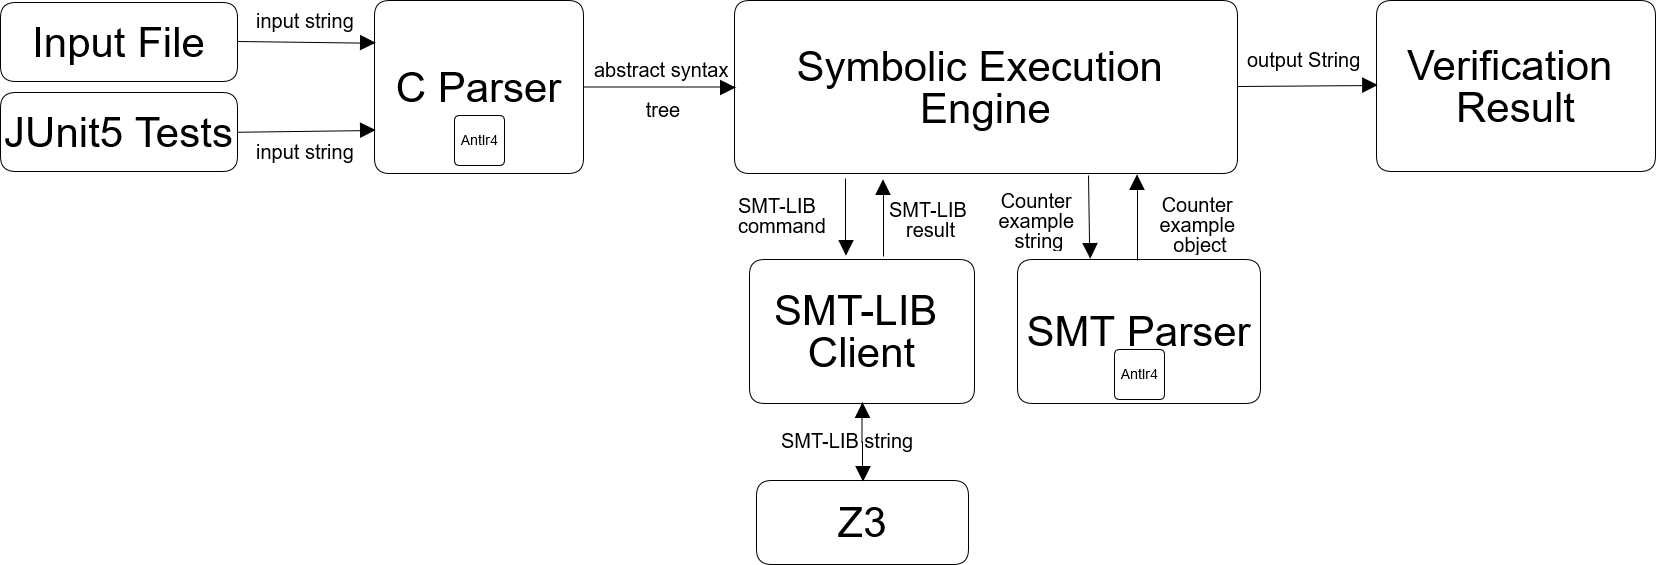
\includegraphics[scale=.25,keepaspectratio=true]{./engine.png}
 % gantt_chart.png: 0x0 pixel, 0dpi, nanxnan cm, bb=
 \caption{Project architecture.}
 \label{fig:engine}
\end{figure}

The project is implemented using Java and the executable is a jar file (target/SymbolicEngine.jar) which is generated using the command:
\definecolor{light-gray}{gray}{0.95}
\lstset{backgroundcolor= \color{light-gray}}

\begin{lstlisting}  
mvn install
\end{lstlisting}  

The program receives as an input a source file containing a simple C function. For testing, \textbf{JUnit5} was used to test the program directly using 45 unit tests. The input (from the input file or the unit test) is passed to the \textbf{C Parser} which uses the ANTLR library to parse the input into an abstract syntax tree. This abstract syntax tree is consumed by the \textbf{Symbolic execution engine} which executes statements and evaluates expressions symbolically to build assertion formulas which are encoded in SMT-LIB commands. These commands are passed to the \textbf{SMT-LIB client} which interacts with the SMT solver Z3.  
Z3 results are passed to \textbf{Symbolic execution engine} through \textbf{SMT-LIB Client}. Z3 counter examples are handled by the \textbf{SMT Parser}. Finally the \textbf{Symbolic execution engine} returns the verification results which include a validity answer for each formula: \textbf{Yes}, \textbf{No} with a counter example, or \textbf{Unknown}. 


Here is an example of an input:

\definecolor{light-gray}{gray}{0.95}

\lstset{caption={test.txt},backgroundcolor= \color{light-gray}}


\begin{lstlisting}  
void f (int x, int y)
{
    if(x > 0)
    {
        y = x;
    }
    assert (y == x);
}
\end{lstlisting}

Here is the output:

\lstset{caption={java -jar TypeChecker.jar -i test.txt}}

\begin{lstlisting} 
Total Answer: No
----------------
Assertions: assert(BinaryExpression: Variable: y==Variable: x;)
AssertionFormula:
(assert (> _x1 0))
(assert (not (= _x1 _x1)))
Answer: Yes
----------------------------
AssertionFormula:
(assert (not (> _x1 0)))
(assert (not (= _x2 _x1)))
Answer: No
Counter example: {x=0, y=1}
----------------------------

\end{lstlisting} 

The following sections focus on the symbolic execution engine. 

\subsection{Symbolic execution engine} \label{sec:execution}


\section{Work Division} 

Since there is only one person in this project, all the work is done by him. 

\bibliographystyle{plain}

\bibliography{references}

\end{document}
